
\chapter{Results and Discussion}

The simulator capture sets of five perspective images and converts them into one image, mimicking the effect of Fisheye lenses cameras. Using the setup described in Section~\ref{sec:combining_pictures}, and an calibratable polynomial lens model, each images is mapped onto specific parts of the final fisheye image. In Figure~\ref{fig:res_show_fisheye} the complete image is shown, simulating a $270^\circ$ FoV camera, mounted beneath the multirotor during flight. 

\begin{figure}[!htb]
    \centering
    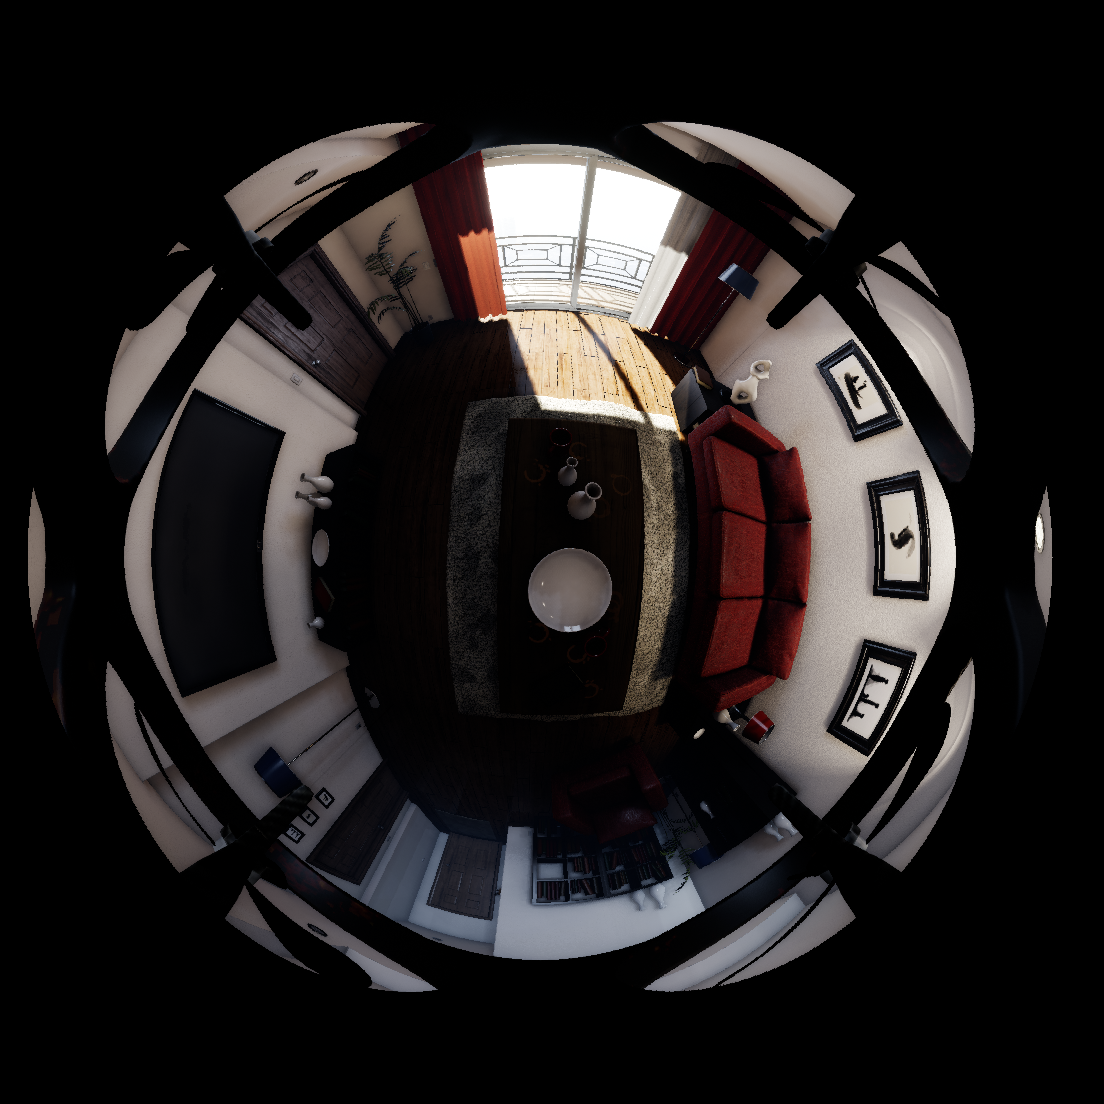
\includegraphics[width=0.7\textwidth]{rapport/fig/Results/1024to2048.png}
    \caption{Simulated fisheye image taken in an indoor environment in Unreal Engine}
    \label{fig:res_show_fisheye}
\end{figure}

\section{Results}

The simulator is able to capture either single $90^\circ$ Fov pictures or full $270^\circ$ FoV pictures. The resolution settings for the perspective images can be set to a maximum of $4096\times4096$, and while there is no current limit to the resolution of the fisheye image, the height and width should should not exceed the double of the input image sizes. The FOV must equal $90^\circ$ for cube capture, but can be both increased and decreased for single captures, as long as the spect ratio is preserved. 

\begin{figure}[!htb]
    \centering
    \begin{subfigure}{0.45\textwidth}
        \centering
        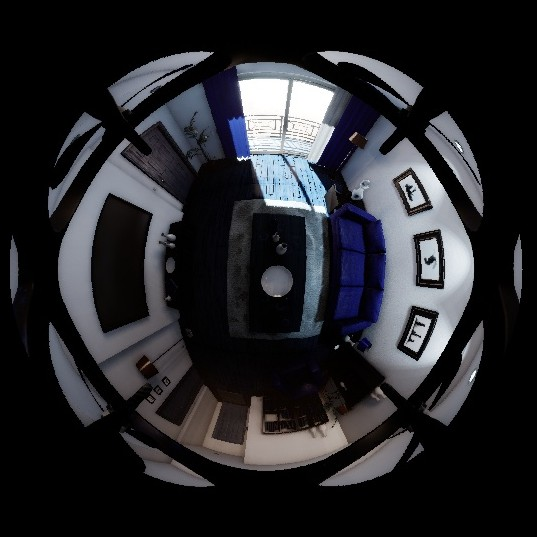
\includegraphics[height=7cm]{rapport/fig/Results/wrongcolor.jpeg}
        \caption{RGBA color}
        \label{fig:res_wrong_color}
    \end{subfigure}
    \begin{subfigure}{0.45\textwidth}
        \centering
        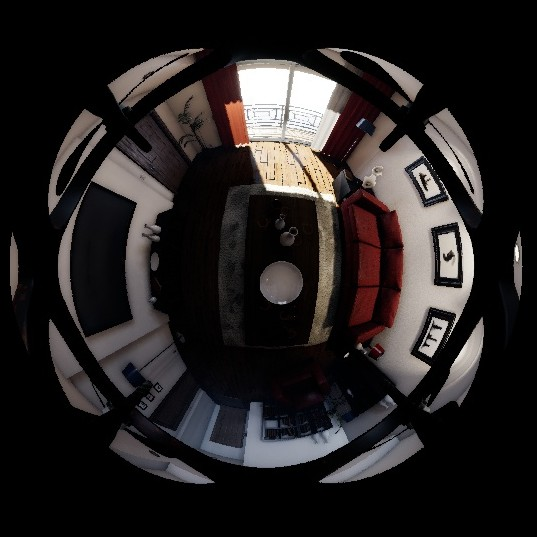
\includegraphics[height=7cm]{rapport/fig/Results/rightcolor.jpeg}
        \caption{BGRA color}
        \label{fig:res_rigth_color}
    \end{subfigure}
    \caption{The effects of pixel ordering}
    \label{fig:res_RGBA_BGRA}
\end{figure}

\begin{figure}[!htb]
    \centering
    \begin{subfigure}{0.32\textwidth}
    \centering
        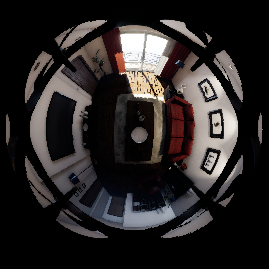
\includegraphics[height=5cm]{rapport/fig/Results/256to512.png}
        \caption{$512 \times 512$ pixels}
        \label{fig:res_comp_256_to_512}
    \end{subfigure}
    \begin{subfigure}{0.32\textwidth}
        \centering
        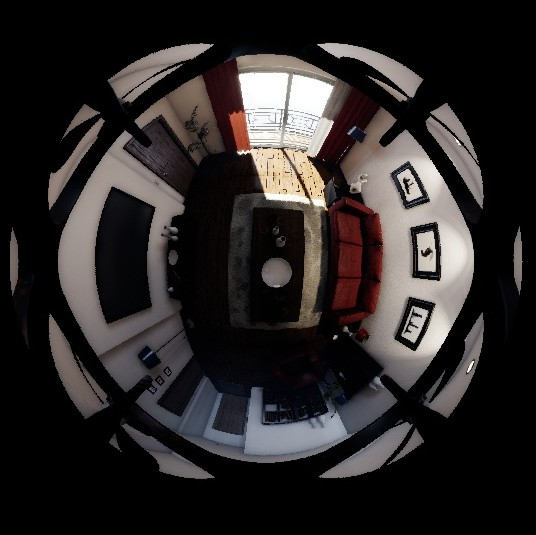
\includegraphics[height=5cm]{rapport/fig/Results/512to1024.jpeg}
        \caption{$1024 \times 1024$ pixels}
        \label{fig:res_comp_512_1024}
    \end{subfigure}    
    \begin{subfigure}{0.32\textwidth}
        \centering
        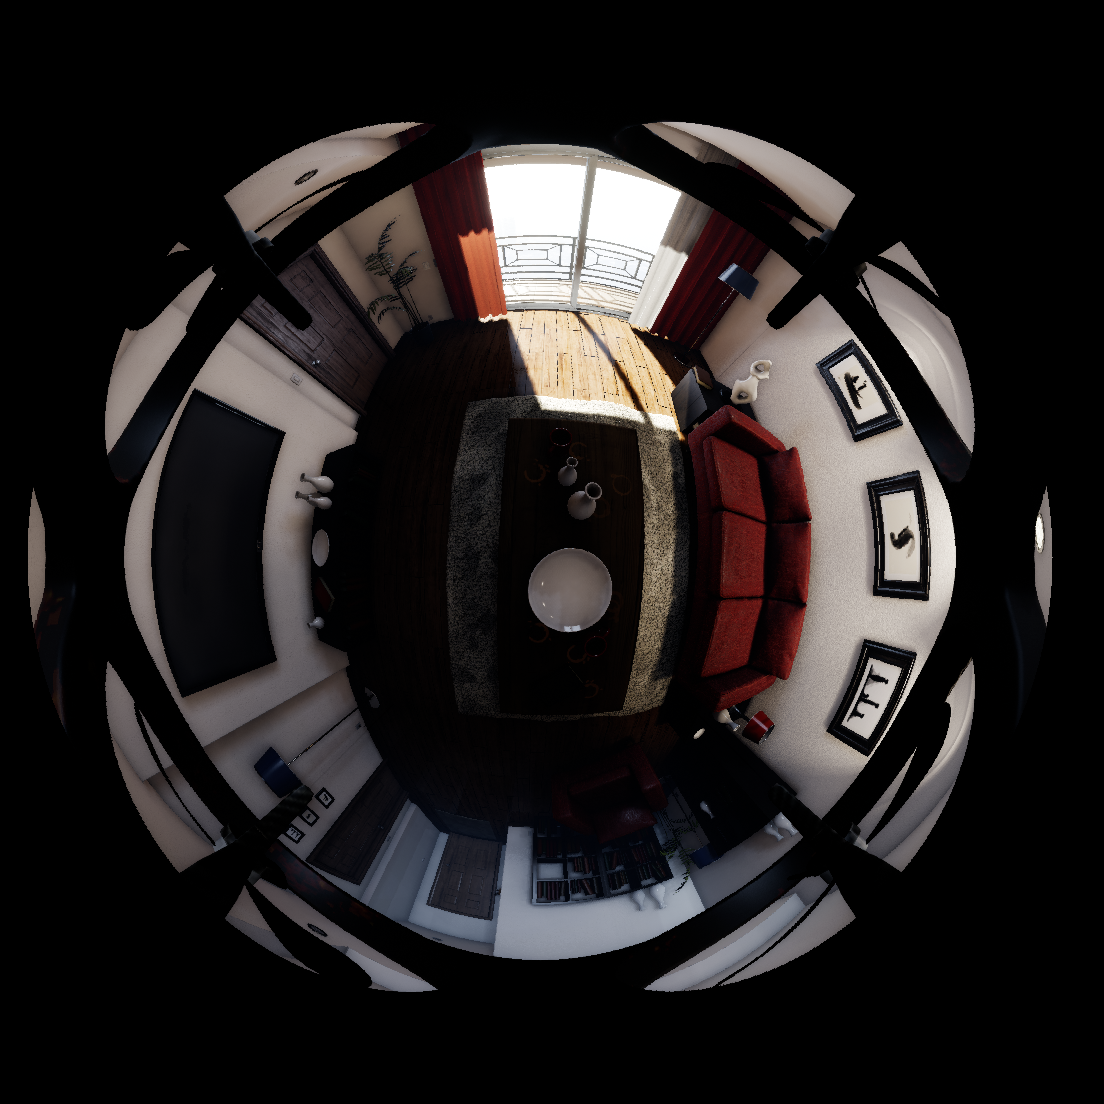
\includegraphics[height=5cm]{rapport/fig/Results/1024to2048.png}
        \caption{$2048 \times 2048$ pixels}
        \label{fig:res_comp_1024_2048}
    \end{subfigure}
    \centering
    \caption{Comparison of image quality in different resolutions}
    \label{fig_res_quality_comparison}
\end{figure}

\begin{figure}[!htb]
    \centering
    \begin{subfigure}{0.32\textwidth}
    \centering
        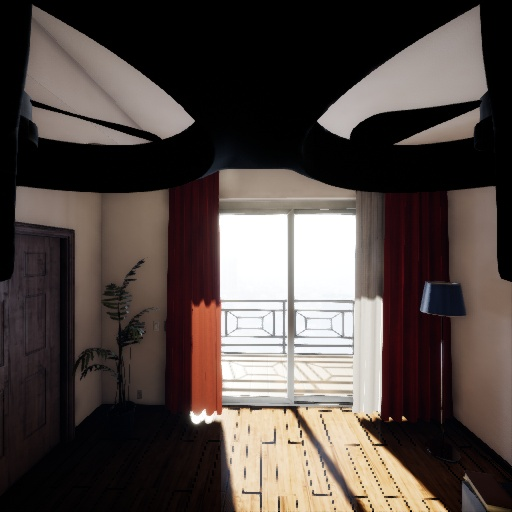
\includegraphics[height=5cm]{rapport/fig/Results/forward_center.jpeg}
        \caption{Front Camera}
        \label{fig:res_original_front}
    \end{subfigure}
    \begin{subfigure}{0.32\textwidth}
        \centering
        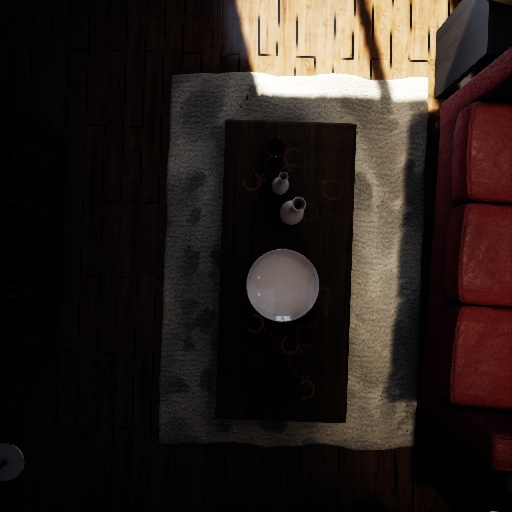
\includegraphics[height=5cm]{rapport/fig/Results/down_center.jpeg}
        \caption{Downward camera}
        \label{fig:res_original_down}
    \end{subfigure}    
    \begin{subfigure}{0.32\textwidth}
        \centering
        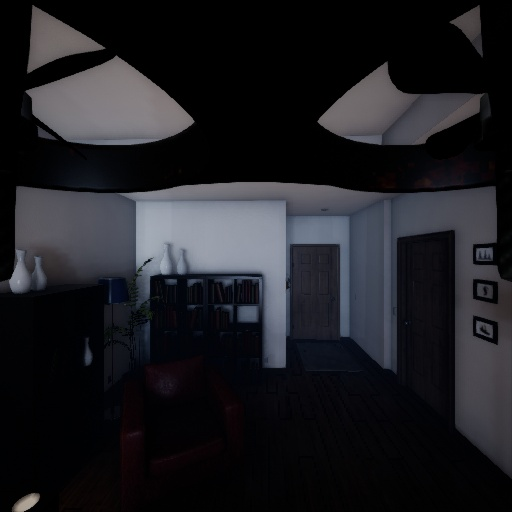
\includegraphics[height=5cm]{rapport/fig/Results/backward_center.jpeg}
        \caption{Back camera}
        \label{fig:res_original_back}
    \end{subfigure} \\[0.75ex]
    \begin{subfigure}{0.32\textwidth}
        \centering
        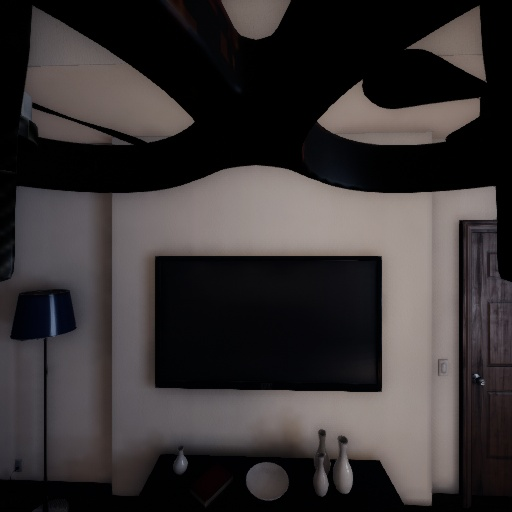
\includegraphics[height=5cm]{rapport/fig/Results/left_center.jpeg}
        \caption{Right camera}
        \label{fig:res_original_left}
    \end{subfigure}    
    \begin{subfigure}{0.32\textwidth}
        \centering
        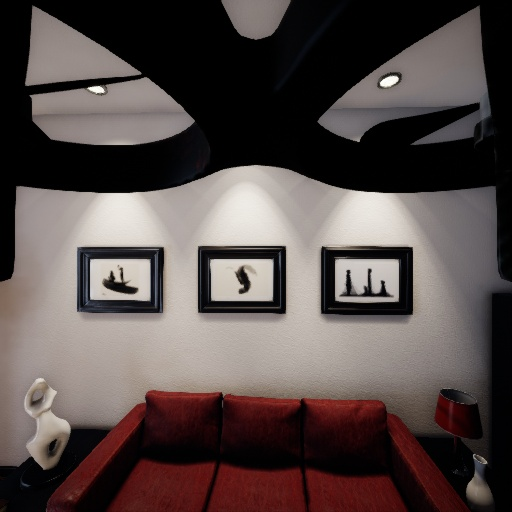
\includegraphics[height=5cm]{rapport/fig/Results/right_center.jpeg}
        \caption{Left Camera}
        \label{fig:res_original_right}
    \end{subfigure}
    \centering
    \caption{Comparison of image quality in different resolutions}
    \label{fig:res_original_pictures}
\end{figure}

\subsection{performance}



\subsection{compile time and runtime calculations}



\subsection{optimization}



\subsection{Discussion}

The task of creating the simulator has been much larger than anticipated at the start of this project. 

\subsection{Image Quality}

\subsection{Performance and optimization}

\subsection{Task}

This project has not been a typical cybernetics project, and in many ways it shares more similarities with a computer science project. While the goal of was to extend the project to incorporate calibrating the fisheye camera to an actual camera, and possiby test computer vision algorithms on the platform, there hasn't been time. This is mainly because of lack of experience in critical areas. 

The project has had to handle very large code bases. Both the codebase of Unreal Engine and AirSim is quite extensive, as they both provide lots of functionality and features. While both platforms have a large user base, few of these discuss problems around the source code and the communication patterns within. Information regarding this is mostly limited to Github issues, and a few forum posts. While these problems became less relevant when making the client side application, it was a huge part of the development described in Section~\ref{sec:Early_dev}. 

Since the fisheye model was to be included into the AirSim interface, a deep understanding of the AirSim package was needed. Both in terms of internal dependencies, class and type definitions, coding style and communication patterns. The fact that it also had to incorporate new funtionality fom Unreal Engine meant that knowledge of C++ scripting towards Unreal Engine was needed. As the platform has an enormous amount of tools and funtionality available, there are also a lot of abstractions, to make the interface possible to use and develop for. However, the lack of previous experiece with game engines or Unreal Engine in particular, made this process quite time consuming. While reading through guides and watching tutorials

\subsection{Platform}

% This decision was made in order to separate the implementation into its own module, and thereby reducing the impact of changes to AirSim. As AirSim is still developed heavilly upon, it was seen as a way to reduce the amount trouble induced by changes to the core code of the plugin. This would also allow me to more often integrate the bug fixes and new implementations they made, without ruining my ownw work. The downside of this decision is that it removes possibility to use any features in Unreal Engine which is not implemented in the AirSim API. 


% \subsection{Project setup and programming environment}

% In this project I have forked both the EpicGames/Unreal Engine and the Microsoft/AirSim repository to my Github account, and made my own pivate repository for the project. This enable me to do specific changes to the source code of these projects, without the need to make pull requests to their original repositories. While AirSim is openly available, the source code of Unreal Engine is only available after being registered as a developer through their website. One requirement for getting the source code is that it is not distributed outside of this licencing. For this reason neither the fork of Unreal Engine, nor my own project repository are publicly available.

% Since one of the main goals of this project is the interfacing to ROS, the main OS for development will be Linux, specifically Ubuntu 18.04. However, since Unreal Engine is deeply integrated with Visual Studios, I will use Visual Studios on Windows as the main debugging platform, for everything except ROS. To build on Linux, I will use CMake, as they have done with AirSim. Both Unreal Engine and AirSim is built with the clang compiler, using libc++ as the standard library. However, the default ROS install uses libstdc++ as their standard library. This caused linking problems when combining ROS and AirSim. I therefore had to make some changes to the build and CMake scripts of AirSim in order to build with the GNU compiler g++, using libstdc++ as the standard library.

% \todo[inline]{Do I need to describe why this change is important?}

\cleardoublepage